\subsection{Metropolis Algorithm}\label{metrop}
At each iteration, the Hastings/Gibbs sampling algorithm \citep{hastings1970,gelfand1992} proposes values for parameters of interest (those with priors in Equation~\ref{eqn:bigproblem}). The algorithm accepts or rejects proposed sets of parameter values by comparison between the proposed and previously-accepted settings, as measured a the log-likelihood or ``cost". A low cost value represents good agreement between model and observations. According to the Hastings/Gibbs algorithm, if the cost associated with proposed parameters is lower than that of the last accepted iteration, the proposed parameter values are accepted. Alternatively, higher cost values may be accepted with a probability determined by the change in likelihood. Both likelihood functions must result in acceptance in order for the proposed parameters to be accepted.


There are two likelihood functions, describing the model-data misfit in reflector depth and age, respectively:

\begin{equation}\label{eqn:loglikedepth}
p(TWTT_r | D_r,d_{firn},v_{ice} ) \propto exp[\frac{-\sum_{r=4}[TWTT_{r} - TWTT_{m,r}(D_r)]^2}{2\sigma_{TWTT}^2}]
\end{equation}

\begin{equation}\label{eqn:loglikeage}
p(A_{IC} | D_{IC},\vec{f},S) \propto exp[\frac{-S\sum_{j = 61}[A_{IC,j} - A_{m,j}(\vec{f},D_{IC})]^2}{2\sigma_A^2} + R^6]
\end{equation}


In the depth likelihood function, $TWTT_m(D_r)$ is based on the relationship between estimates of $D_r$ and TWTT as in Equation~\ref{deptheqn}. $TWTT_r$ is observed by ice-penetrating radar for each reflector, $r$. Uncertainty in TWTT, $\sigma_{TWTT}$, is taken to be 14 ns due to intrinsic errors in the precision of the radar system as described in the previous section.

%To estimate $\sigma_{TWTT}$, we assume a perfect model and compute with standard deviation of the numerator given typical errors we expect affect our data. This method allows for correlation between depth errors, as expected. More details are discussed in the Supplement.


In the age likelihood function, the modeled age, $A_m$, is a function of ice flow model parameters and accumulation rate history, $\vec{f}$. A regularization term, $R^6$, is used to penalize large variability in the accumulation rates input to the ice flow model and $A_m$ comes from solutions to the forward ice flow model. We use $J=61$ volcanic events from \citet{hammer1997} as the observational target, $A_{IC}$, which do not include uncertainty information. These data represent dated volcanic deposits observed in the Byrd ice core and extend to $\sim$ 50 ka, though there is a lack of data in the brittle zone of the ice core between 300 and 900 m depth, where the electrical conductivity cannot be continuously measured \citep{hammer1997}. To determine volcanic age uncertainties, we include a precision parameter, $S$, and use it to infer uncertainty in the volcanic record from scatter between our model and the observed data. $S$ is a ``nuisance" parameter that accounts for uncertainty in $\sigma_A$ by using $E_m$ as a measure of scatter between modeled age $A_m$ and $p(S) \sim Ga(\alpha,\beta)$ \citep{jackson&huerta2016}. The posterior probability distribution of $S$ is:

\begin{equation}\label{eqn:S}
PPD(S) = Ga(\frac{k_e}{2}+\alpha, E_m+\beta)
\end{equation}
where 
\begin{equation}
 E_m= \frac{\sum_{j}[A_{IC,j} - A_{m,j}(\vec{f},D_{IC})]^2}{2\sigma_A^2} 
\end{equation}

Parameters $\alpha$ and $\beta$ are assumed to be 1 as in the case for a noninformative gamma prior. Unlike other parameters in our problem, values of $S$ are proposed using Gibbs sampling \citep{gelfand1992}, effectively estimating reflector age uncertainty given the choice of ice flow model parameters for each iteration.

The number of degrees of freedom, $k_e$, is not known. We assume it is less than $J$ because it is reasonable that errors in age and depth are related within the ice column. Here we guess assume $k_e = \frac{j}{2}$ = 30.5, which assumes there are strong correlations among age solutions. The solution uncertainty is affected by the value of $k_e$ as shown by the the sensitivity of our results to our choice of $k_e$ in Figure~\ref{fig:ke}. We find that our choice does not significantly impact the mean estimates of age or depth for our radar reflectors. %In lieu of independent information about an appropriate value of $k_e$, we choose to assume $k_e = \frac{J}{2} = 30.5$ because mixing of the accumulation rate parameters is strong and the rate at which the algorithm finds solutions is reasonable. 

\begin{figure*}[ht]
\begin{center}
%\centering
\makebox[\textwidth][c]{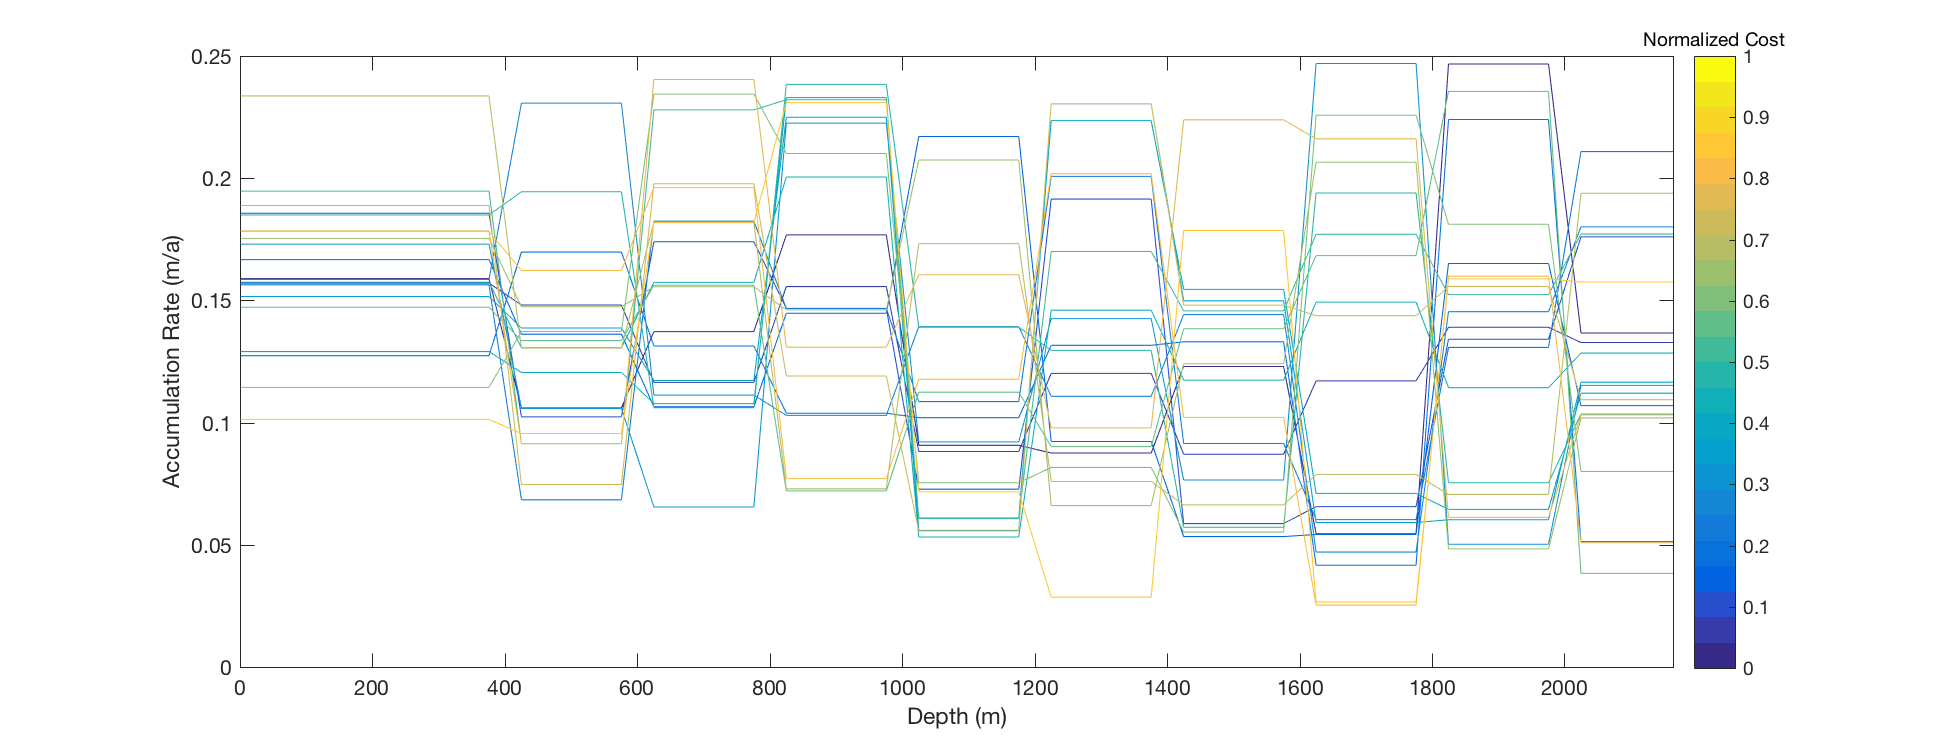
\includegraphics[scale=0.35]{../analysis/figures/keCompare}}
%\captionsetup{width=.9\textwidth}
\caption[scale=0.3]{Comparison of reflector age for different degrees of freedom, $k_e$. The choice of $k_e$ has an effect on uncertainty in reflector age estimates, but does not greatly impact mean estimates. }
\end{center}
\label{fig:ke}
\end{figure*}


%The Metropolis algorithm randomly samples each of the ice flow parameters and computes an age-depth profile. A Bayesian method is used to determine suitability of proposed ice flow parameters in a Bayesian way:
%\begin{equation}\label{posterior}
% p(\vec{f},\sigma_V | A_V, D_V) \propto p(A_V,D_V | \vec{f},\sigma_V) p(\vec{f}) p(\sigma_V),
%\end{equation}
%A posterior probability, $p(A | \vec{f})$, is computed for each set of parameters from likelihood and prior probabilities, $P(\vec{f})$. As described below, we require only the proportional relation because relative posterior values are considered in this Markov Chain process.

%The simulated age-depth profile is compared to the observed volcanic chronology using the ``log-likelihood" function, $p(A_V,D_V | \vec{f},\sigma_V)$, to quantify how closely a sampled set of parameters represents the observed ice profile:
%
%\begin{equation}\label{cost}
%ln(likelihood) = \frac{1}{N}\sum\frac{(A_{sim}(\vec{f})_i~ - ~A_{V,i})^2}{(2\sigma_{V})^2},
%\end{equation}
%where $\vec{Age}_{sim}$ comes from evaluating the ice flow model for parameter values sampled from $\vec{f}$. $A_{V}$ and $\sigma_{V}$ describe the observed volcanic chronology at the Byrd ice core. The prior on $\sigma_{V}$ is 
%\begin{equation}
%p(\sigma_V) \sim Ga(\alpha, \beta)
%\end{equation}

%which assumes error in the chronology is $\sim$3\% (T.J. Fudge, pers. comm.). Uncertainty in the volcanic chronology, $\sigma_{V}$, loosens the constraint on how closely $A_{sim}$ must match $A_{V}$ to be acceptable. We assume $N$ degrees of freedom, where $N$ is the number of volcanic observations. This is because observed global volcanic events are assumed independent.
%


